%!TEX TS-program = xelatex
%!TEX encoding = UTF-8 Unicode

\documentclass[12pt]{extarticle}
% extarticle is like article but can handle 8pt, 9pt, 10pt, 11pt, 12pt, 14pt, 17pt, and 20pt text

\def \ititle {Origins of Mind}
 
\def \isubtitle {Lecture 07}
 
\def \iauthor {Stephen A. Butterfill}
\def \iemail{s.butterfill@warwick.ac.uk}
\date{}

%for strikethrough
\usepackage[normalem]{ulem}

\input{$HOME/Documents/submissions/preamble_steve_handout}

%\bibpunct{}{}{,}{s}{}{,}  %use superscript TICS style bib
%remove hanging indent for TICS style bib
%TODO doesnt work
\setlength{\bibhang}{0em}
%\setlength{\bibsep}{0.5em}


%itemize bullet should be dash
\renewcommand{\labelitemi}{$-$}

\begin{document}

\begin{multicols}{3}

\setlength\footnotesep{1em}


\bibliographystyle{newapa} %apalike

%\maketitle
%\tableofcontents




%--------------- 
%--- start paste
\def \ititle {Origins of Mind}
 
\def \isubtitle {Lecture 07}
 
 
 
\
 
 
 
\begin{center}
 
{\Large
 
\textbf{\ititle}: \isubtitle
 
}
 
 
 
\iemail %
 
\end{center}
 
 
 
\section{Knowledge of Mind}
 
\textit{Mindreading} is the process of identifying mental states and purposive actions as the mental states and purposive actions of a particular subject.
 
‘In saying that an individual has a theory of mind, we mean that the individual imputes mental states to himself and to others’
\citep[p.\ 515]{premack_does_1978}
 
In a standard \textit{false belief task}, `[t]he subject is aware that he/she and another person [Maxi] witness a certain state of affairs x. Then, in the absence of the other person the subject witnesses an unexpected change in the state of affairs from x to y' \citep[p.\ 106]{Wimmer:1983dz}. The task is designed to measure the subject's sensitivity to the probability that Maxi will falsely believe x to obtain.
 
 
 
\section{Mindreading: First Puzzle}
 
\subsection{Theory of mind cognition is hard}
 
Conceptually demanding:
 
\begin{itemize}\itemsep0pt
 
\item Acquisition takes several years \citep{Wimmer:1983dz,Wellman:2001lz}
 
\item Tied to the development of executive function \citep{Perner:1999yr,Sabbagh:2006ke} and language \citep{Astington2005ot}
 
\item Development facilitated by explicit training \citep{Slaughter:1996fv} and siblings \citep{Clements:2000nc,Hughes:2004zj}
 
\end{itemize}
 
Cognitively demanding:
 
\begin{itemize}
 
\item Requires attention and working memory in fully competent adults \citep{Apperly:2008jv,McKinnon:2007rr}
 
\end{itemize}
 
 
 
\section{Mindreading: Second Puzzle}
 
Are human adults’ abilities to represent beliefs automatic?
 
There is evidence for \citep{kovacs_social_2010,Schneider:2011fk} and against \citep{apperly:2008_back,apperly_why_2010}.
 
 
 
\section{Modules and Cognitive Efficiency}
 
How could mindreading ever (but not always) be automatic?
 
Representing perceptions and beliefs as such---and even merely holding in mind what another believes, where no inference is required---involves a measurable processing cost\citep{apperly:2008_back,apperly:2010_limits}, consumes attention and working memory in fully competent adults,\citealp{Apperly:2009cc, lin:2010_reflexively, McKinnon:2007rr} may require inhibition\citep{bull:2008_role} and makes demands on executive function.\citep{apperly:2004_frontal,samson:2005_seeing}
 
 
 
\section{Minimal Theory of Mind}
 
An agent’s \emph{field} is a set of objects related to the agent by proximity, orientation and other factors.
 
First approximation: an agent \emph{encounters} an object just if it is in her field.
 
A \emph{goal} is an outcome to which one or more actions are, or might be, directed.
 
%(Not to be confused with a \emph{goal-state}, which is an intention or other state of an agent linking an action to a particular goal to which it is directed.)
 
\textbf{Principle 1}: one can’t goal-directedly act on an object unless one has encountered it.
 
Applications: subordinate chimps retrieve food when a dominant is not informed of its location \citep{Hare:2001ph}; when observed scrub-jays prefer to cache in shady, distant and occluded locations \citep{Dally:2004xf,Clayton:2007fh}.
 
First approximation: an agent \emph{registers} an object at a location just if she most recently encountered the object at that location.
 
A registration is \emph{correct} just if the object is at the location it is registered at.
 
\textbf{Principle 2}: correct registration is a condition of successful action.
 
Applications: 12-month-olds point to inform depending on their informants’ goals and ignorance \citep{Liszkowski:2008al}; chimps retrieve food when a dominant is misinformed about its location \citep{Hare:2001ph}; scrub-jays observed caching food by a competitor later re-cache in private \citep{Clayton:2007fh,Emery:2007ze}.
 
\textbf{Principle 3}: when an agent performs a goal-directed action and the goal specifies an object, the agent will act as if the object were actually in the location she registers it at.
 
Applications: some false belief tasks \citep{Onishi:2005hm,Southgate:2007js,Buttelmann:2009gy}.
 
 
 
\section{Signature Limits Generate Predictions}
 
\begin{center}
 
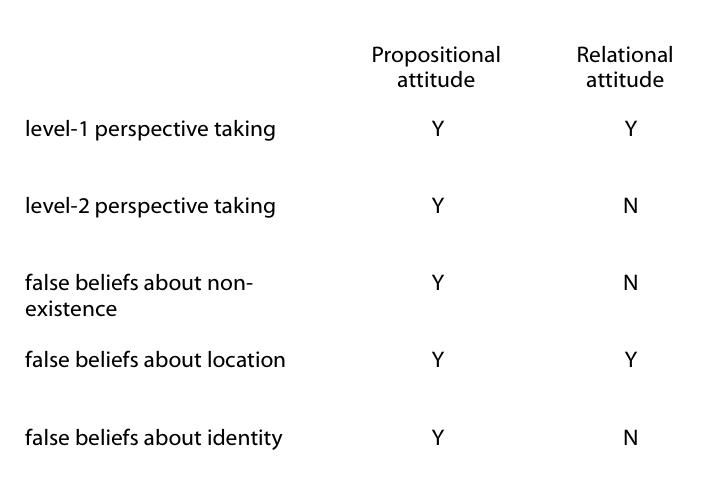
\includegraphics[width=0.25\textwidth]{fig/signature_limits_table.png}
 
\end{center}
 
\begin{center}
 
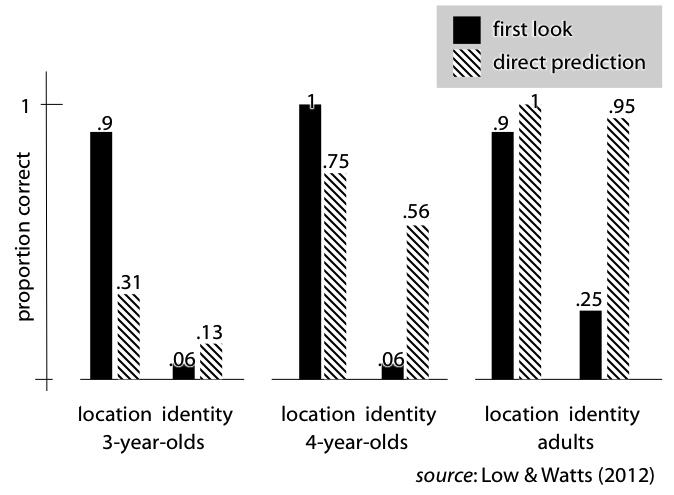
\includegraphics[width=0.3\textwidth]{fig/low_2012_fig.png}
 
\end{center}
  
 
%--- end paste
%--------------- 
 
\footnotesize 
\bibliography{$HOME/endnote/phd_biblio}

\end{multicols}

\end{document}